\chapter{Validación y resultados}

\noindent
En esta sección se muestran los resultados obtenidos después de la implementación. En 
primer lugar se realizaron un conjunto de pruebas para validar que el sistema tuviera las 
propiedades deseadas. Se validó que el último módulo, la búsqueda en árbol de información 
perfecta, calculara jugadas con buen desempeño. Asímismo, se corrieron simulaciones para 
tener una idea sobre la sensibilidad de los parámetros de MCTS. Por último se muestra el 
desempeño del sistema y se contrasta con los requerimientos y restricciones planteadas al 
inicio del escrito.

\section{Validación de MCTS}

A lo largo del desarrollo, la metodología de  \textit{Test Driven Development} fue útil para ganar 
certidumbre sobre el correcto funcionamiento del programa. Aun así, contar con pruebas 
unitarias no asegura que las partes del sistema funcionen correctamente en conjunto. 
Después de integrar las reglas de dominó con MCTS, era necesario validar que el resultado 
de la búsqueda fuera una jugada con buen desempeño. 

Para verificar el funcionamiento del último módulo se simularon mil juegos de dominó con 
las fichas abiertas entre un equipo MCTS y un equipo greedy. 

\begin{figure}[ht]
\begin{center}
\hbox{\hspace{-1em} 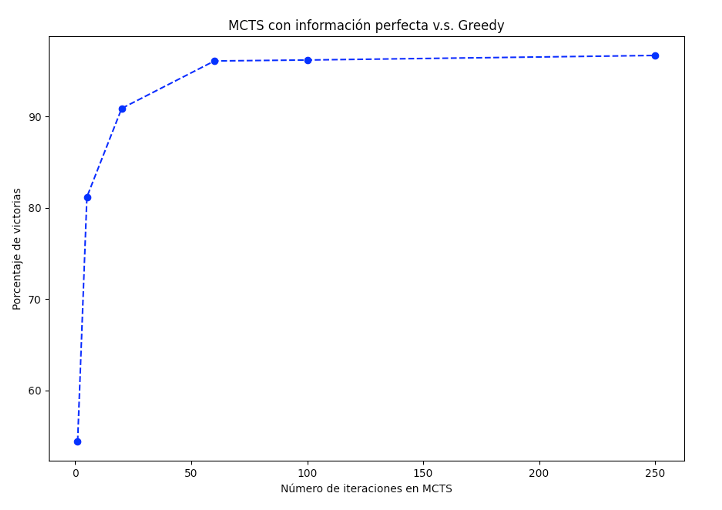
\includegraphics[scale=0.9]{mcts_greedy_abierto.png}}
\caption{MCTS v.s. Greedy. MCTS vence en más del 90\% de los juegos con 50 simulaciones de MCTS}
\label{MGA}
\end{center}
\end{figure}

En la figura \ref{MGA} tenemos una gráfica del resultado de las simulaciones. En el eje 
horizontal se muestra el número de iteraciones que se le permitió ejecutar a MCTS para 
cada tiro. Se corrieron seis simulaciones con distintas configuraciones de MCTS de mil 
juegos cada una. Podemos observar que muy rápidamente se llega a superar al equipo 
greedy. Con menos de 20 iteraciones, la búsqueda en árbol logró vencer al jugador greedy 
en 80\% de los juegos. La gráfica sugiere que el desempeño del equipo MCTS converge 
cuando se le permiten 90 iteraciones a la búsqueda.

El desempeño observado nos indica que MCTS está calculando buenas jugadas y que el 
módulo funciona correctamente.

\section{Sensibilidad de MCTS a su parámetro de búsqueda}

El resultado anterior sugería que con noventa iteraciones la decisión de MCTS converge. Si 
sucediera así, la decisión que toma MCTS sería la misma sin importar si se corre con 
noventa iteraciones o más y dos equipos contrincantes MCTS con parámetros distintos 
deberían tener el mismo desempeño y ganar en 50\% de los juegos cada uno. Se puso a 
prueba esta hipótesis simulando juegos entre un equipo con número de iteraciones fija 
(250) contra un equipo de parámetro variable. Se corrieron las simulaciones para ocho 
valores distintos del parámetro de búsqueda.

\begin{figure}[ht]
\begin{center}
\hbox{\hspace{-1.5em} 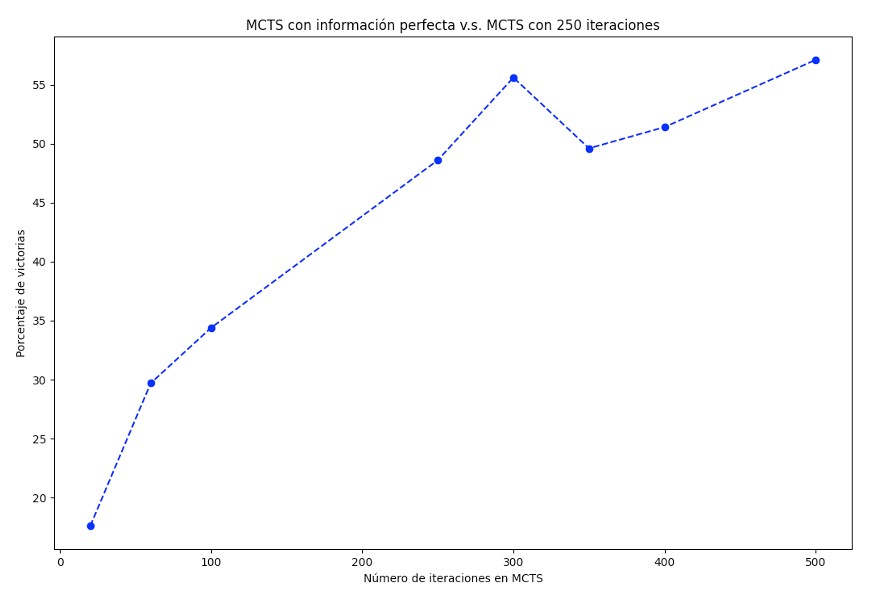
\includegraphics[scale=0.85]{mcts_mcts_250.png}}
\caption{MCTS v.s. MCTS con 250 iteraciones. El desempeño del algoritmo es sensible al parámetro de búsqueda}
\label{MM250}
\end{center}
\end{figure}


De la figura \ref{MM250}, se puede notar que la hipótesis era incorrecta. A pesar de que el 
desempeño de MCTS contra greedy no es sensible al parámetro con valores mayores a 
noventa, el desempeño general sigue dependiendo del parámetro. Un equipo MCTS con 
doscientas cincuenta iteraciones tiene mejor desempeño que un equipo con menos 
iteraciones.

De lo anterior se deduce que cuando se compite contra un equipo greedy no es necesario 
correr muchas iteraciones en MCTS para calcular buenas jugadas pero es posible que el 
desempeño sea menor contra jugadores más fuertes. La figura 4 también sugiere que MCTS 
converge a partir de las doscientas cincuenta iteraciones, pues los puntos posteriores oscilan 
alrededor del 50\%, comportamiento que se esperaría de equipos con desempeño igual. 
Inclusive al duplicar las iteraciones a quinientos no parece haber cambio significativo en el 
porcentaje de victorias.

\section{Desempeño del sistema}

El análisis anterior fue útil para encontrar una combinación de parámetros adecuada para 
satisfacer los requerimientos y las restricciones del problema. El sistema necesita que se 
definan dos parámetros. El número de iteraciones de búsqueda y el número de escenarios 
que se simulan. Ya que el desempeño de MCTS contra greedy no requería un gran número 
de iteraciones, se decidió correr veinte iteraciones de MCTS por cada escenario. Por otro 
lado, se eligió simular cien escenarios por tiro.

Se simularon mil juegos de dominó (donde cada jugador sólo conoce sus fichas) entre el 
equipo PIMC contra un equipo greedy. El sistema consiguió 74\% de victorias y el tiempo 
que tomó en cada tirada fue de 1.2 segundos corriendo en el servidor de Digital Ocean.